%\documentclass[10pt, conference, compsocconf]{IEEEtran}
\documentclass{article}
\usepackage{times}
\usepackage{xcolor}
\usepackage{mathtools}
\usepackage{enumerate}
\usepackage{hyperref}
\usepackage{amssymb}
\usepackage{subfig}
\usepackage{amsmath}
\usepackage{eqnarray}
\usepackage[]{algorithm}
\usepackage{clrscode3e}
\usepackage[pdftex]{graphicx}
\usepackage{amsthm}

\DeclarePairedDelimiter{\ceil}{\lceil}{\rceil}

\newtheorem{lemma}{Lemma}
\newtheorem{theorem}{Theorem}

\begin{document}

%%%%%%%%%%%%%%%%%%%%%%%%%%%%%%%%%%%%%%%%%%%%%%%%%%%%%%%%%%%%%%%%%%%%%%%
%%%%%%%%%%%%%%%%%%%%%%%%%%%%%%%%%%%%%%%%%%%%%%%%%%%%%%%%%%%%%%%%%%%%%%%
%%
%% TITLE
%%
%%%%%%%%%%%%%%%%%%%%%%%%%%%%%%%%%%%%%%%%%%%%%%%%%%%%%%%%%%%%%%%%%%%%%%%
%%%%%%%%%%%%%%%%%%%%%%%%%%%%%%%%%%%%%%%%%%%%%%%%%%%%%%%%%%%%%%%%%%%%%%%

\title{Hierarchical watershed segmentation of graphs}

\author{
Aleksandar Zlateski\\ Massachusetts Institute of Technology\\ Cambridge, MA\\
{\tt\small zlateski@mit.edu}
\and
H. Sebastian Seung\\ Princeton University\\ Princeton, NJ\\
{\tt\small sseung@princeton.edu}
}



\maketitle
%\thispagestyle{empty}

%%%%%%%%%%%%%%%%%%%%%%%%%%%%%%%%%%%%%%%%%%%%%%%%%%%%%%%%%%%%%%%%%%%%%%%
%%%%%%%%%%%%%%%%%%%%%%%%%%%%%%%%%%%%%%%%%%%%%%%%%%%%%%%%%%%%%%%%%%%%%%%
%%
%% ABSTRACT
%%
%%%%%%%%%%%%%%%%%%%%%%%%%%%%%%%%%%%%%%%%%%%%%%%%%%%%%%%%%%%%%%%%%%%%%%%
%%%%%%%%%%%%%%%%%%%%%%%%%%%%%%%%%%%%%%%%%%%%%%%%%%%%%%%%%%%%%%%%%%%%%%%


\begin{abstract}
We present a new definition and algorithm for hierarchical watershed
segmentation of an affinity graph.  Our algorithm computes a directed
graph that defines a unique direction of steepest ascent for every
vertex in the affinity graph.
% Every steepest ascent path is guaranteed to converge to a regional maximum of the affinity graph, and escape from any plateau through the closest plateau corner.
The basins of attraction of the steepest ascent dynamics constitute a
flat segmentation.  The result is similar to ``watershed cuts,''
except that plateaus are divided in a systematic and even manner.
Applying single linkage clustering to the watershed basins yields a
hierarchy of segmentations.  We prove that this is a ``natural''
definition of hierarchy, in the sense that each of its levels is
equivalent to the flat watershed segmentation of some upper
thresholding of the original affinity graph. The time complexity
scales quasilinearly with the number of edges, making our algorithm
practical even for very large graphs.

\end{abstract}

%%%%%%%%%%%%%%%%%%%%%%%%%%%%%%%%%%%%%%%%%%%%%%%%%%%%%%%%%%%%%%%%%%%%%%%
%%%%%%%%%%%%%%%%%%%%%%%%%%%%%%%%%%%%%%%%%%%%%%%%%%%%%%%%%%%%%%%%%%%%%%%
%%
%% INTRODUCTION
%%
%%%%%%%%%%%%%%%%%%%%%%%%%%%%%%%%%%%%%%%%%%%%%%%%%%%%%%%%%%%%%%%%%%%%%%%
%%%%%%%%%%%%%%%%%%%%%%%%%%%%%%%%%%%%%%%%%%%%%%%%%%%%%%%%%%%%%%%%%%%%%%%

\section{Introduction}
Many interesting computational problems can be formulated as the
partitioning or segmentation of a weighted undirected graph.  The
weight of an edge between two vertices represents their ``affinity'' for each other (cite).  High affinity indicates that the vertices should be in
the same segment, and low affinity indicates that the vertices should
be in different segments.  This statement has been formalized by
various objective functions, and many algorithms have been studied for
optimizing the objective functions.  Polynomial time algorithms are of
practical interest.  For very large graphs, it would be desirable to
have an algorithm that runs in linear time or close-to-linear time.
Only a few of these have been proposed.  One example is the
``watershed cuts'' algorithm \cite{Cousty2009,Cousty2010}.

Here we provide a new algorithm for watershed segmentation of graphs.
As in watershed cuts, the algorithm utilizes a dynamical system that
is discrete in space and time.  The dynamical system steps from pixel
to pixel while taking a path of steepest ascent on the pixel values.
The basins of attraction of the dynamics constitute the resulting
segmentation.

The main motivation is to handle the division of plateaus in a
systematic way. The watershed definition becomes subtle in the
presence of plateaus.  In these ``flat'' parts of a graph, the
direction of steepest ascent is not uniquely defined.  Our algorithm
divides plateaus evenly, in the sense that the dynamics follows the
shortest path to escape from any plateau.

The watershed cuts algorithm alternates between depth first search
(DFS) and breadth first search (BFS) for an attractor of the gradient
descent dynamics.  It starts with DFS, switches to BFS when it enters
a plateau, and switches back to DFS when it exits a plateau, and
continues alternating in this way until an attractor is found.

Our algorithm splits the search process into several passes through
the graph.  The first pass explicitly computes a steepest ascent
graph.  The second pass divides plateaus via BFS. The third pass finds
connected components.

Like watershed cuts, our algorithm has linear time complexity.  The
use of multiple passes makes it possible to divide plateaus evenly.  A
second motivation for our algorithm is that it separates the
computation into two passes that are parallelizable versus two passes
that are not.  A parallel variant of our algorithm will be described
in a future paper.

Watershed segmentation typically generates too many segments, because
every local maximum gives rise to a watershed basin.  The number of
local maxima can be reduced by smoothing the graph before the
watershed algorithm is applied.  A simple smoothing method is to set
all affinities above a threshold $\theta$ to infinity.

Varying $\theta$ gives rise to a family of watershed segmentations.  We show that this hierarchy is equivalent to single linkage clustering of watershed basins. 

\section{Flat segmentation}
Consider a connected graph $G=(V,E)$ with non-negative edge
weights. An edge $\{u,v\}$ is \emph{locally maximal} for
$u$ if there is no other edge incident to $u$ with higher weight.  A
\emph{steepest ascent path} $\left\langle
v_{0},e_{0},v_{1},e_{1},v_{2}, \dots \right\rangle$ is one
for which every edge $e_{i}$ is locally maximal with respect to
$v_{i}.$

A \emph{regional maximum} $M$ is a connected subgraph of $G$ such that
there is a steepest ascent path between any pair of vertices in $M$,
and every steepest ascent path starting in $M$ will
stay within $M$. A vertex $v$ belongs to the \emph{basin of
  attraction} of a \emph{regional maximum $M$} if there exists a
steepest ascent path from $v$ to any vertex in $M$.

In the special case where all edge weights take on unique values, the
locally maximal edge is uniquely defined for each vertex.  It follows
that the steepest ascent path from every vertex is uniquely defined,
and that every vertex belongs to exactly one basin of
attraction.\footnote{Every basin consists of two vertices, and the
  steepest ascent path within a basin cycles between the two
  vertices.}  The basins form a partition of the graph, which is
defined as the output of the watershed transform.

[describe standard algorithms for finding the basins.  MST, Prim, Kruskal. disjoint sets ]

More generally, a locally maximal edge for a vertex may not be unique,
because of the possibility of ties.  It follows that a steepest
ascent path starting from a vertex may not be unique, and that a
vertex may belong to more than one basin of attraction.  Furthermore,
there may exist steepest ascent paths that never converge to a
regional maximum but remain stuck on non-maximal ``plateaus.''  In
this case, the definition of the watershed transform is more subtle.

[describe watershed cuts]

Our algorithm explicitly computes a new directed graph $D_1$ from the
original undirected graph $G$.  The edges of $D_1$ are the steepest
ascent edges of $G$, and the paths of $D_1$ are the steepest ascent
paths of the original graph.  Then edges are eliminated from $D_1$ to
create $D_2$, in which all steepest ascent paths (1) converge to
regional maxima, (2) are unique outside regional maxima, and (3)
divide plateaus evenly.

\begin{figure}
  \centering
  \subfloat[]{\protect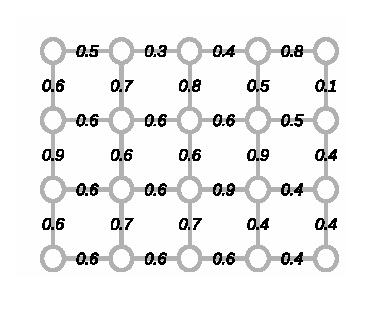
\includegraphics[scale=0.66]{fig/affinity_graph}}
  \subfloat[]{\protect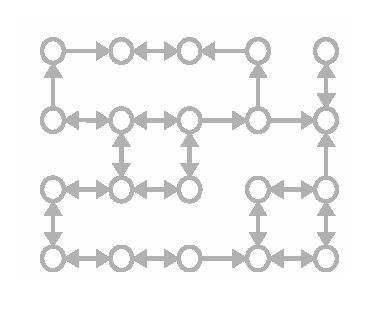
\includegraphics[scale=0.66]{fig/sd_graph}}\\
  \subfloat[]{\protect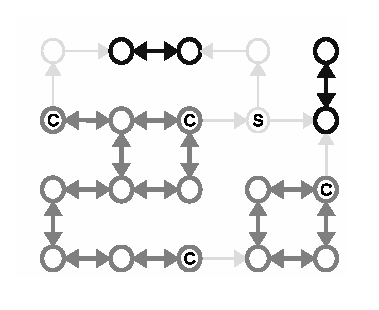
\includegraphics[scale=0.66]{fig/sd_graph_plateaus}}
  \subfloat[]{\protect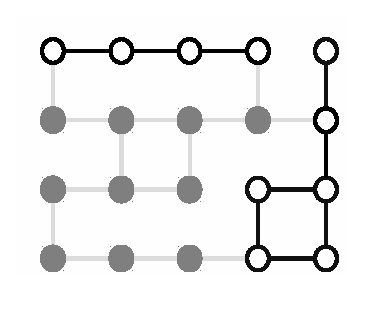
\includegraphics[scale=0.66]{fig/ws_result}}

  \protect\caption{(a) A disaffinity graph; (b) derived steepest
    descent graph; (c) locally minimal plateaus (black), non-minimal
    plateau (dark gray), saddle vertex (S), plateau corners (C); (d)
    the two basins of attractions and border vertices (dark gray)}
\end{figure}

\subsection{Steepest ascent graph}
The starting point is an undirected weighted graph $G$.  Replace each
edge of $G$ by edges in both directions between the same vertices
(Fig. 1(a)).  Then for every vertex retain the outgoing edge with
maximal weight and eliminate other outgoing edges.  The resulting
directed unweighted graph is called $D_1$.

If there are ties between outgoing edges (Fig. 1b), they are resolved
by assuming a pre-existing ordering of the vertices.  The ordering
could be represented by a bijective map
$\alpha:V\to\{1,2,...,|V|\}$. We refer to $\alpha(u)$ as the index of
$u$ (Fig. 2a).  The winning edge is the one pointing to the vertex
with the lowest index.

If a pair of vertices has edges in both directions, they are
represented by a single ``bidirectional edge'' in Fig. 1b, and we will
use this term for convenience.  Threrefore, the edges of any vertex in
$D_1$ can be classified as incoming, outgoing, and bidirectional.

A directed path in $D_1$ is a path of steepest ascent in $G$.

A steepest descent graph can be defined analogously using edges of
minimal weight. Either steepest ascent or descent can be used without
loss of generality.

\begin{figure}
  \centering
  \subfloat[]{\protect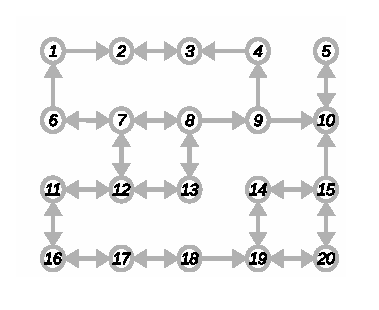
\includegraphics[scale=0.66]{fig/sd_graph_ordered}}
  \subfloat[]{\protect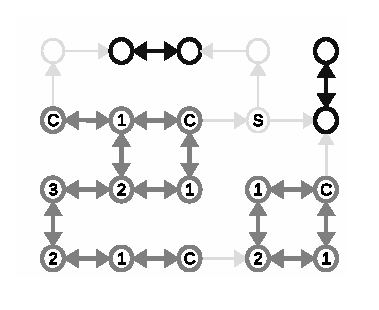
\includegraphics[scale=0.66]{fig/sd_graph_plateaus_ordered}}\\
  \subfloat[]{\protect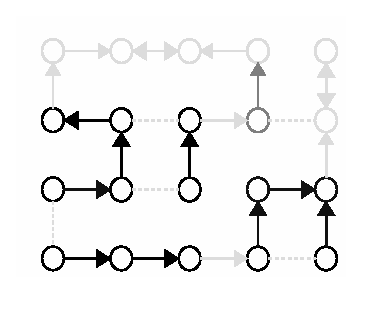
\includegraphics[scale=0.66]{fig/sd_graph_plateaus_modified}}
  \subfloat[]{\protect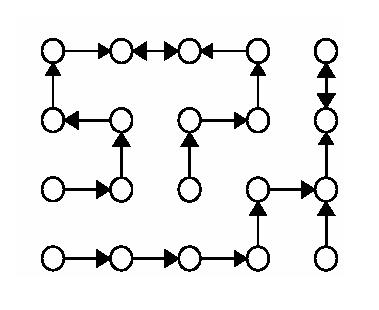
\includegraphics[scale=0.66]{fig/final_segmentation}}

  \protect\caption{(a) Vertex indices; (b) distances to the nearest
    plateau corner; (c) modifications to the steepest descent graph;
    (d) final watershed partition of the graph}
\end{figure}

\subsection{Plateau division}
While no vertex in $D_1$ has two or more outgoing edges, directed
paths are still not uniquely defined, because of the existence of
plateaus.  A \emph{plateau} is a connected component of the subgraph
of $D_1$ containing only bidirectional edges.  A plateau \emph{corner}
is a plateau vertex with an outgoing edge.
% there can't be more than one, since saddles were eliminated, right?
\emph{Locally maximal} plateaus contain no corners; they are
equivalent to the regional maxima of the original graph.  If a
directed path of $D_1$ enters a locally maximal plateau, it remains
within the plateau for all future time.

\emph{Non-maximal} plateaus contain one or more corners.  If a
directed path enters a non-maximal plateau, it may stay within the
plateau, or exit through one of the corners.  These types
of plateaus are illustrated in Fig. 1c.

We would like to alter $D_1$ so that any directed path that enters a
non-maximal plateau will not get stuck there, but will eventually
exit.  This guarantees that any directed path will eventually reach a
regional maximum, i.e., regional maxima are attractors of the dynamics.

Furthermore, we would like a non-maximal plateau with multiple corners
to be divided evenly, in the following sense.  From each vertex in the
plateau, the directed path should lead to the nearest corner, where
nearest is defined based on graph distance.  If there is a tie between
corners, it should be resolved using the same ordering function as
before.  Both of these goals are achieved for a non-maximal plateau by
performing a breadth first search (BFS) for all of its vertices,
starting from its corners with the canonical ordering.

The BFS proceeds as follows.  We initialize a global FIFO queue $Q$,
mark all the corner vertices as visited and insert them into $Q$ in
increasing order of their index. While $Q$ is not empty we remove the
vertex $v$ from the front of the queue, and loop over all its
bidirectional edges $\{v,u\}$.  If $u$ has not yet been visited, we
mark it as visited, insert it to the back of the queue, and change the
edge from bidirectional to incoming $(v\leftarrow u)$. If $u$ has
already been visited, we remove the bidirectional edge $\{v,u\}$
completely.

\subsection{Connected components}
After applying this BFS to every non-maximal plateau, we arrive at the
modified steepest ascent graph $D_2$ (Fig. 2c).  Every directed path eventually reaches a locally maximal plateau.  The path from any vertex to its corresponding regional maximum is unique.  Therefore, the graph can be segmented into the basins of attraction of the dynamics.

The basins can be found by regarding $D_2$ as an undirected graph and
computing its connected components.  [via what algorithm]

\subsection{Time complexity}
As we operate on a connected graph we assume $O(|E|) \ge O(|V|)$.  To
create $D_1$, we visit each edge a constant number of times. To create
$D_2$, we visit each vertex at most once, and edges incident to it a
constant number of times. The complexity of connected components is
$O(|E|)$.  Therefore the overall complexity is $O(|E|)$.

\subsection{Properties of watershed segmentation}
The algorithm produces an optimal partitioning as defined
in~\cite{Cousty2009}.

Basins are in one-to-one correspondence with regional maxima.

maximal spanning forest
steepest ascent graph in each basin is maximal spanning tree?

\section{Hierarchical segmentation}
Many methods have been proposed for turning a flat watershed
segmentation into a hierarchical segmentation.  Most methods amount to
some kind of agglomerative clustering algorithm applied to the
watershed basins.  Such algorithms define an affinity function for
pairs of clusters, and merge the pair with highest affinity at each
step.  Many affinity functions have been proposed
\cite{Najman1996}(cite Beucher and others).  Here we propose single
linkage clustering for defining the hierarchy.  Given that this is a
relatively simple and perhaps even naive method, its performance may
not be competitive with more sophisticated methods. However, single
linkage clustering is worth considering because it is (1) efficiently
computable and (2) leads to a definition of hierarchy that is
particularly ``natural,'' in a way that will be made precise below.

\subsection{Single linkage clustering}
In single linkage clustering, the affinity of two clusters is defined
as the maximal affinity of all edges between the two clusters.  At
each step, a pair of clusters with maximum affinity is merged.  The
output is a dendrogram.  The height of each branch point is given by
the affinity at which the two clusters merge.

[describe efficient algorithm and its time complexity]

% maximin affinity between two regional maxima in two clusters

\subsection{Upper thresholding of the affinity graph}
Above we claimed that single linkage clustering leads to a definition
of hierarchy that is particularly ``natural'' for watershed.  The
rationale for this claim is as follows.  Suppose that the original
affinity graph were modified by replacing all affinities larger than
$\theta_{\max}$ by a common high value (e.g. $\infty$).  The flat watershed
segmentation of the modified affinity graph would correspond to one of
the levels of the hierarchical segmentation produced by single linkage
clustering.

To prove this, we first prove the following lemma:
\begin{lemma}
  Let $G'$ be the affinity graph obtained by setting all affinities of
  $G$ greater than $\theta$ to a common high value (e.g. $\infty$).
  Let $W=\{B_1,B_2,\dots\}$ and $W'=\{B'_1,B'_2,\dots\}$ be the
  watershed segmentations of $G$ and $G'$, respectively.  For each
  $B_i$ there exists $B'_j$ such that $B_i \subseteq B'_j$.
\end{lemma}

\begin{proof}
Let $S_2$ and $S_2'$ be the steepest ascent graphs obtained from $G$
and $G'$, respectively.  Vertices of $S_2$ not incident to any edge
with affinity smaller than $\theta$ will stay unmodified, even after
plateau division. All other vertices of $S_2$ will become part of a
locally maximal plateau of $S_2'$ (regional maximum of $G'$). All
locally maximal edges of $S_2$ will stay locally maximal. Therefore
the only effect of the affinity threshold is to introduce
bidirectional edges. Therefore, a connected component of $S_2$ has to
be a subset of a connected component of $S_2'$
\end{proof}

Now we are ready to prove the following theorem.
\begin{theorem}
The following are equivalent:
\begin{enumerate}
\item Watershed segmentation of $G$ followed by single linkage clustering of the basins up to affinity $\theta$.
\item Creation of $G'$ from $G$ by replacing all affinities larger
  than $\theta$ by a common high value (e.g. $\infty$), followed by
  watershed segmentation of $G'$.
\end{enumerate}
\end{theorem}

\begin{proof}
  Watershed basins of $W'$ are connected. Hence, they can be obtained by
merging watershed basins of $W$. We prove that the result of 1. and
2. are equivalent by showing that two neighboring basins of $W$, $B_i$
and $B_j$ will be merged in 1. if and only if they are merged in 2.

Let's examine two watershed basins of $W$, $B_i$ and $B_j$. If there
is an edge $\{u,v\}$ in $G$ such that $u \in B_i$ and $v \in B_j$ with
the weight smaller than $T_{\min}$, then $u$ and $v$ will be part of
the same regional minima in $W'$. Hence, the two basins of $W$ belong
to a single basin of $W'$. We also know that the saliency between
$B_i$ and $B_j$ has to be smaller than $T_{\min}$, therefore they will
belong to the same segment when applying the algorithm 1. Similarly,
if the saliency $d_{ij}$ between $B_i$ and $B_j$ is below $T_{\min}$,
then there exist an edge $\{u,v\}$ in $G$ such that $u \in B_i$ and $v
\in B_j$ with the weight equal to $d_{ij} < T_{\min}$. Therefore $u$
and $v$ will be part of the same regional minima, and $B_i$ and $B_j$
will be part of the same watershed basin in $W'$.
\end{proof}

\section{Source code}
3D image
Nearest neighbor affinity graph 

\section{Discussion}
To show confidence about high values of \emph{disaffinities}, and in
order to prevent undesired mergers, we introduce a threshold
$\theta_{\min}$ by eliminating all edges with affinity less than
$\theta_{\min}$. The lower threshold can produce singleton vertices in
$G$. The singleton vertices are not assigned to any watershed basin
and are considered background, which is often a desired result.

mention possible improvements to hierarchy

%%%%%%%%%%%%%%%%%%%%%%%%%%%%%%%%%%%%%%%%%%%%%%%%%%%%%%%%%%%%%%%%%%%%%%%
%%%%%%%%%%%%%%%%%%%%%%%%%%%%%%%%%%%%%%%%%%%%%%%%%%%%%%%%%%%%%%%%%%%%%%%
%%
%% REFERENCES
%%
%%%%%%%%%%%%%%%%%%%%%%%%%%%%%%%%%%%%%%%%%%%%%%%%%%%%%%%%%%%%%%%%%%%%%%%
%%%%%%%%%%%%%%%%%%%%%%%%%%%%%%%%%%%%%%%%%%%%%%%%%%%%%%%%%%%%%%%%%%%%%%%


{\small
\bibliographystyle{ieeetr}
\bibliography{./ref/bib}
}

\end{document}

\subsection{Assigning border vertices}
In Fig. 1(d) we show the \emph{basins of attraction} of the two
\emph{regional minima}. The \emph{border} vertices are shown in dark
gray and belong to both \emph{basins of attraction}. Watershed
cuts~\cite{Cousty2009,Cousty2010} assign \emph{border} vertices with a
single constraint that all the \emph{basins of attraction} have to be
connected.

